\scanpage{67}
% archive foliation: 66
% lines 1--8, letterhead
\begin{minipage}{.45\linewidth}\centering
U N I V E R S I T E\\
DES SCIENCES ET TECHNIQUES\\
DU LANGUEDOC\\
------------\\
Service de la Scolarité\\
MR / GJ\\
Diffusion : Liste A\\
N° : 4066
\end{minipage}\hfill
\begin{minipage}{.48\linewidth}
Montpellier, le 28 Juin 1978
\end{minipage}

% lines 9--10
\begin{center}
\uline{AVIS DE SOUTENANCE D'UNE THESE DE DOCTORAT DE 3ème CYCLE}

\uline{( CHIMIE ORGANIQUE PHYSIQUE )}
\end{center}

% lines 11--14
\uline{Nom et prénom du candidat} :\qquad AURELLY Michèle

\uline{Titre de la thèse} : Application de la corrélation de Hammett à l'étude de
l'énolisation des cétones en milieux basique et superbasique.

% lines 15--17
\uline{Date, heure et lieu de soutenance prévus} :
\begin{flushright}
JEUDI 13 JUILLET 1978 à 16 Heures\\
Salle de cours n° 9 - U. S. T. L.
\end{flushright}

% lines 18--21
\uline{Nom du Directeur de thèse} :
\begin{flushright}Monsieur le Professeur LAMATY.\end{flushright}

\uline{Désignation du laboratoire où la thèse est préparée} :
\begin{flushright}Laboratoire de Chimie Organique Physique.\end{flushright}

% lines 22--27
\uline{Analyse de l'ouvrage} :

Ce travail consiste à cerner de plus près
les mécanismes de l'énolisation des cétones par l'étude d'acétophénones et
de méthyl-2 phényl-1 butanones-1 substituées, dans des milieux basiques.
Les constantes \unsure{$p$|$\rho$} de Hammett ont été mesurées en fonction de la nature du milieu.

% lines 28--34
\uline{Durée approximative des recherches ayant abouti à la thèse : 3 ans.}

\uline{Composition du jury proposé} :
\begin{center}
MM. :\\
LAMATY, Président\\
SCHUE\\
WYLDE\\
MION
\end{center}

% lines 35--37, signature
\begin{flushright}
Le Secrétaire Général,

\figure{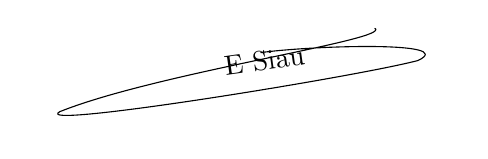
\begin{tikzpicture}[x=1cm,y=1cm]
\node[rotate=8] at(2.7,.6){\unsure{E Siau}};
\draw(4.1,1.01)..controls(4.35,.87)and(1.35,.45)..(.1,-.05)
..controls(-.3,-.28)and(3.85,.39)..(4.65,.6)
..controls(5.18,.85)and(3.3,.79)..(2.65,.7);
\end{tikzpicture}}

\uline{E. SIAU}
\end{flushright}
